 
\begin{center}
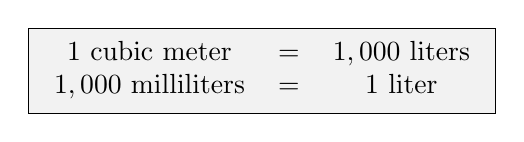
\begin{tikzpicture}
\draw(0,0)node[draw=black, fill=black!5!white, rectangle]{\begin{tabular} {ccc}
$1$ cubic meter &$=$& $1,000$ liters \\
$1,000$ milliliters &$=$& $1$ liter 
\end{tabular}};
\end{tikzpicture}
\end{center}
A chemical factory makes deionized water in $10$ cubic meter batches, which then are packaged in bottles containing $250$ milliliters each.  Based on the information given in the box above, how many $250$ milliliter bottles are there in one $10$ cubic meter batch?\\ \\
\begin{tabular}{lrcl}
A)\hspace{3mm}& 400,00&\hspace{-4mm}0& \\
B)\hspace{3mm}& 40,00&\hspace{-4mm}0&\\
C)\hspace{3mm}& 4,00&\hspace{-4mm}0&\\
D)\hspace{3mm}&&\hspace{-4mm}0&\hspace{-4mm}.0004\\
\end{tabular}\\ \\


\ifsat
	\begin{enumerate}[label=\Alph*)]
	\end{enumerate}
\else
\fi

\ifacteven
	\begin{enumerate}[label=\textbf{\Alph*.},itemsep=\fill,align=left]
		\setcounter{enumii}{5}
		\item None of these. 
	\end{enumerate}
\else
\fi

\ifactodd
	\begin{enumerate}[label=\textbf{\Alph*.},itemsep=\fill,align=left]
		\item None of these. 
	\end{enumerate}
\else
\fi

\ifgridin
\else
\fi

